% Build: tectonic main.tex   (or: pdflatex main && bibtex main && pdflatex main && pdflatex main)
% Every number in this file is taken from the released result files (results/*.json, results/SUMMARY.md). Rows and
% numbers marked "NCM paper" are quoted from arXiv 2610.14162. Figures: scripts/fig_*.py (data), figures/method.tex.
% Layout: the LaTeX template of the NCM paper (arXiv 2610.14162).

% fix-cm lets the Computer Modern fonts scale to any size (used for the 19 pt title)
\RequirePackage{fix-cm}
\documentclass[11pt]{article}
\ifdefined\XeTeXversion\else\pdfoutput=1\fi
\usepackage[T1]{fontenc}
\usepackage[expansion=false]{microtype}% same line breaks under pdfLaTeX and XeTeX
\usepackage{graphicx}
\usepackage{float}
\usepackage{booktabs}
\usepackage{amssymb}
\usepackage{amsmath}
\usepackage[table]{xcolor}
\usepackage{multirow}
\usepackage[margin=1in]{geometry}
\usepackage{authblk}
\usepackage[numbers]{natbib}
\usepackage{array}
\usepackage{placeins}
\usepackage{needspace}% start a paragraph on the next page when only a few lines of this one are left
\usepackage{enumitem}
\usepackage{caption}
\usepackage{fontawesome5}  % GitHub icon (\faGithub) for the code link under the title
% let LaTeX stretch interword space a little in paragraphs that would otherwise run into the margin
\setlength{\emergencystretch}{3em}
% Avoid ending a paragraph with the isolated tail of a hyphenated word.
\finalhyphendemerits=1000000

\usepackage{tikz}
\usetikzlibrary{arrows.meta,calc,positioning}

% Hyperlink colours: blue for references and citations, pink for URLs
\definecolor{linkblue}{RGB}{38,110,165}
\definecolor{linkpink}{HTML}{EC008C}
% colours of the method schematic (figures/method.tex)
% (as in the figures of the NCM paper: gold for the codes the generator produces, darker for coarser levels; blue for
% the context that is kept)
\definecolor{cgold}{HTML}{EDA100}\definecolor{cgoldtxt}{HTML}{7A5200}\definecolor{cgoldedge}{HTML}{B07A0A}
\definecolor{cgoldbg}{HTML}{FFF8E6}
\definecolor{clvA}{HTML}{B87A00}\definecolor{clvB}{HTML}{E09A0E}\definecolor{clvC}{HTML}{F5BA3E}
\definecolor{clvD}{HTML}{FAD48A}\definecolor{clvE}{HTML}{FDEBC0}
\definecolor{cctx}{HTML}{7FA6D6}\definecolor{cctxedge}{HTML}{6F93C2}\definecolor{cctxtxt}{HTML}{5578A5}
\definecolor{cink}{HTML}{1F1F1E}\definecolor{cmuted}{HTML}{6B6A63}
% highlight of the proposed rows in the tables
\definecolor{oursrow}{HTML}{FFF1CC}

\usepackage[
  colorlinks=true,
  linkcolor=linkblue,
  citecolor=linkblue,
  urlcolor=linkpink,
  filecolor=linkblue,
  bookmarks=true,
  bookmarksopen=true
]{hyperref}

% No first-line indent; paragraphs are separated by vertical space.
\usepackage[parfill]{parskip}

% floats: up to two at the top of a page, and enough text allowed beside them
\renewcommand{\topfraction}{0.88}\renewcommand{\bottomfraction}{0.6}\renewcommand{\textfraction}{0.1}
\renewcommand{\floatpagefraction}{0.8}\setcounter{topnumber}{2}\setcounter{totalnumber}{3}
\widowpenalty=10000 \clubpenalty=10000 \displaywidowpenalty=10000
\newcolumntype{P}[1]{>{\raggedright\arraybackslash}p{#1}}
\newcolumntype{C}[1]{>{\centering\arraybackslash}p{#1}}

\newcommand{\x}{$\times$}

\title{\vspace{-0.5cm}%
  \fontsize{19}{23}\selectfont A Song of Coarse and Fine:\\
  V-Cycles and Soft Decisions for Next-Concept Models}

\author{Tom\'as Rodrigues}
\affil{maqia (\href{https://maqia.ai}{maqia.ai})}

\date{}

\begin{document}

\maketitle

% code link, centred under the affiliation
\vspace{-0.89cm}
{\centering\small\href{https://github.com/maqiaai-lab/ncm-vcycles}{\textcolor{black}{\faGithub}}\enspace\url{https://github.com/maqiaai-lab/ncm-vcycles}\par}
\vspace{4pt}

\begin{abstract}
Next-Concept Modeling (NCM) generates text coarse to fine: one pass down a hierarchy of discrete codes, with a hard
decision at every level and no way back. That is half of a multigrid V-cycle. We study the whole cycle on the released
checkpoints, without training. Going back up, a \emph{V-cycle} re-encodes the draft with the frozen tokenizer, keeps
its coarse levels and regenerates the fine ones. One cycle lowers generative perplexity by 14--22\% on the released
LM1B and TinyStories models against an equal-compute control, and by 8--13\% against temperature tuning at matched
diversity. Going down, a \emph{soft decision} passes the posterior-mean code vector to the next level instead of the
vector of the chosen code, at no extra network evaluation. It raises WMT14 German$\to$English BLEU from 21.7 to 25.2
($+3.5$, 95\% CI [$+3.1$, $+3.8$]) and COMET by 3.7 points: more than classifier-free guidance at twice the compute,
and more than our own minimum-Bayes-risk run at twelve times the compute. XSum ROUGE-2 rises by 0.8 and one-pass
accuracy on hard Sudoku by 3.8 points, each with its setting chosen on separate data. Together, the two put
unconditional LM1B text about a fifth below temperature tuning in perplexity, and with a rule checker and a new
symmetry frame per retry they reach 96.5\% at 14 evaluations per board on hard Sudoku, against 86.2\% in one pass of
12. A diagnosis explains the blend: a stronger translation system's coarse codes are mostly NCM's first or second
choice, yet NCM's likelihood ranks that plan below its own in more than 99\% of sentences, so reranking has nothing to
find. We also report what fails: on translation the V-cycle adds nothing to soft decisions, on Sudoku re-encoding
adds nothing at matched FLOPs, soft decisions at coarse levels ruin sampled text, and too high a temperature
collapses the output.
\end{abstract}

% ------------------------------------------------------------------------------------------------------------------
\section{Introduction}

Next-Concept Modeling (NCM) \citep{kumbong2026ncm} generates a sequence coarse to fine. A frozen multiscale residual
tokenizer turns a text into a few levels of discrete codes, from one code for the whole sequence up to about one code
per token, and a transformer predicts each level in parallel from the levels before it. A pass costs one network
evaluation per level, about ten for a sentence, instead of one per token.

That pass is half of a multigrid V-cycle \citep{brandt1977multigrid,briggs2000multigrid}. A multigrid solver does not
only prolong a coarse solution to the finer grids. It also \emph{restricts} the fine solution back onto the coarse
grids, recomputes the coarse correction from it, and goes down again. NCM takes the downward half once, and takes it
with a hard decision at every level: decoding keeps one code per position, the next level is conditioned on the vector
of that code alone, and nothing that the fine levels write ever returns to the coarse ones. We study the whole cycle
on the released checkpoints, without training, with one change for each direction.

\emph{Up: the V-cycle} (Figure~\ref{fig:method}a). NCM's frozen tokenizer already provides the restriction. We decode a
draft, re-encode it, keep the re-encoded coarse levels and regenerate the fine ones. A cycle that restarts at level
$m$ costs $K-m$ evaluations, and it can be repeated.

\emph{Down: soft decisions} (Figure~\ref{fig:method}b,\,c). At every position of level $k$ the generator outputs a
distribution over the codebook, and the hard decision discards all of it but the top code. How sure the generator was
and what its second choice would have been are lost, and a wrong coarse code is inherited by every finer level. We
let level $k$ contribute the \emph{posterior-mean code vector} instead, the probability-weighted average of its
codebook. NCM's levels add up to one continuous latent, so this average is a point of the space that the next level
and the decoder already read. The change is one line of the decoder and adds no network evaluation. In decoding theory
it is a \emph{soft decision}: later stages receive the expected symbol instead of a committed one
\citep{wang1999iterative,skoglund1999soft}.

\begin{figure}[t]
\centering
\resizebox{\linewidth}{!}{% Method schematic (TikZ): a V-cycle (a); one level of the downward pass under a hard decision (b) and a soft decision (c).
% Visual language of the schematics of the NCM paper: sans-serif labels, gold for the codes the generator produces
% (darker for coarser levels), blue for the context that is kept.
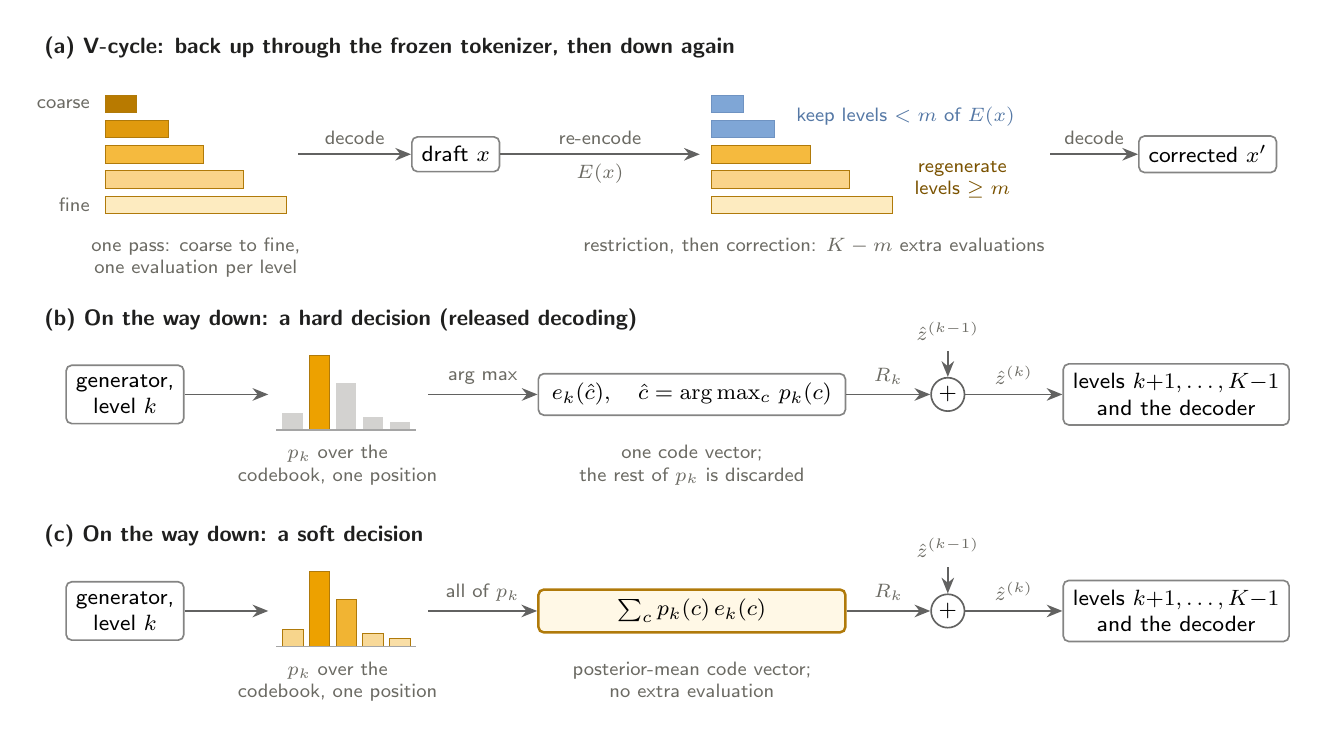
\begin{tikzpicture}[
  font=\sffamily\footnotesize, line width=0.6pt,
  >={Stealth[length=2mm,width=1.6mm]},
  box/.style={draw=cink!55, rounded corners=2pt, align=center, inner sep=3.5pt, fill=white},
  lab/.style={font=\sffamily\scriptsize, text=cmuted, align=center},
  arr/.style={->, draw=cink!70},
  head/.style={font=\sffamily\footnotesize\bfseries, text=cink, anchor=west},
  lev/.style={line width=0.3pt},
]
% ---------------- (a) V-cycle ----------------
\node[head] at (-0.15, 1.30) {(a) V-cycle: back up through the frozen tokenizer, then down again};
% one pass: five levels, coarse (dark) to fine (light)
\foreach \i/\w/\c in {0/0.40/clvA, 1/0.80/clvB, 2/1.25/clvC, 3/1.75/clvD, 4/2.30/clvE}
  \filldraw[lev, fill=\c, draw=cgoldedge] (0.75, {0.70-\i*0.32}) rectangle ++(\w, -0.22);
\coordinate (s1mid) at (3.05, -0.05);
\node[lab, anchor=east] at (0.68, 0.59) {coarse};
\node[lab, anchor=east] at (0.68, -0.69) {fine};
\node[lab, anchor=north] at (1.9, -0.98) {one pass: coarse to fine,\\one evaluation per level};
\node[box] (x) at (5.2, -0.05) {draft $x$};
\draw[arr] ($(s1mid)+(0.15,0)$) -- node[lab, above] {decode} (x.west);
% after re-encoding: the coarse levels are kept as context, the fine ones are generated again
\foreach \i/\w/\c/\e in {0/0.40/cctx/cctxedge, 1/0.80/cctx/cctxedge, 2/1.25/clvC/cgoldedge, 3/1.75/clvD/cgoldedge,
                         4/2.30/clvE/cgoldedge}
  \filldraw[lev, fill=\c, draw=\e] (8.45, {0.70-\i*0.32}) rectangle ++(\w, -0.22);
\coordinate (s2in) at (8.45, -0.05);
\draw[arr] (x.east) -- node[lab, above] {re-encode} node[lab, below] {$E(x)$} ($(s2in)+(-0.15,0)$);
\node[lab, anchor=west, text=cctxtxt] at (9.40, 0.43) {keep levels $<m$ of $E(x)$};
\node[lab, anchor=west, text=cgoldtxt] at (10.90, -0.37) {regenerate\\levels $\geq m$};
\node[box] (xp) at (14.75, -0.05) {corrected $x'$};
\draw[arr] (12.75, -0.05) -- node[lab, above] {decode} (xp.west);
\node[lab, anchor=north] at (9.75, -0.98) {restriction, then correction: $K-m$ extra evaluations};

% ---------------- (b) hard decision ----------------
\begin{scope}[yshift=-3.35cm]
\node[head] at (-0.15, 1.20) {(b) On the way down: a hard decision (released decoding)};
\node[box] (ga) at (1.0, 0.25) {generator,\\level $k$};
\foreach \i/\h in {0/0.22, 2/0.60, 3/0.16, 4/0.10}
  \fill[cmuted!30] ({3.0+\i*0.34}, -0.20) rectangle ++(0.26, \h);
\filldraw[lev, fill=cgold, draw=cgoldedge] ({3.0+0.34}, -0.20) rectangle ++(0.26, 0.95);
\draw[cink!40] (2.92, -0.20) -- (4.70, -0.20);
\node[lab, anchor=north] at (3.70, -0.27) {$p_k$ over the\\codebook, one position};
\draw[arr] (ga.east) -- (2.82, 0.25);
\node[box, minimum width=3.9cm] (va) at (8.2, 0.25) {$e_k(\hat c),\quad \hat c=\arg\max_c\,p_k(c)$};
\draw[arr] (4.85, 0.25) -- node[lab, above] {arg max} (va.west);
\node[lab, anchor=north] at (8.2, -0.27) {one code vector;\\the rest of $p_k$ is discarded};
\node[circle, draw=cink!70, inner sep=1.2pt] (pa) at (11.45, 0.25) {$+$};
\draw[arr] (va.east) -- node[lab, above] {$R_k$} (pa.west);
\node[lab] (za) at (11.45, 1.05) {$\hat z^{(k-1)}$};
\draw[arr] (za.south) -- (pa.north);
\node[box] (na) at (14.35, 0.25) {levels $k{+}1,\dots,K{-}1$\\and the decoder};
\draw[arr] (pa.east) -- node[lab, above] {$\hat z^{(k)}$} (na.west);
\end{scope}

% ---------------- (c) soft decision ----------------
\begin{scope}[yshift=-6.10cm]
\node[head] at (-0.15, 1.20) {(c) On the way down: a soft decision};
\node[box] (gb) at (1.0, 0.25) {generator,\\level $k$};
\foreach \i/\h/\c in {0/0.22/cgold!45, 1/0.95/cgold, 2/0.60/cgold!80, 3/0.16/cgold!40, 4/0.10/cgold!35}
  \filldraw[lev, fill=\c, draw=cgoldedge] ({3.0+\i*0.34}, -0.20) rectangle ++(0.26, \h);
\draw[cink!40] (2.92, -0.20) -- (4.70, -0.20);
\node[lab, anchor=north] at (3.70, -0.27) {$p_k$ over the\\codebook, one position};
\draw[arr] (gb.east) -- (2.82, 0.25);
\node[box, minimum width=3.9cm, draw=cgoldedge, fill=cgoldbg, line width=0.9pt] (vb) at (8.2, 0.25) {$\sum_c p_k(c)\,e_k(c)$};
\draw[arr] (4.85, 0.25) -- node[lab, above] {all of $p_k$} (vb.west);
\node[lab, anchor=north] at (8.2, -0.27) {posterior-mean code vector;\\no extra evaluation};
\node[circle, draw=cink!70, inner sep=1.2pt] (pb) at (11.45, 0.25) {$+$};
\draw[arr] (vb.east) -- node[lab, above] {$R_k$} (pb.west);
\node[lab] (zb) at (11.45, 1.05) {$\hat z^{(k-1)}$};
\draw[arr] (zb.south) -- (pb.north);
\node[box] (nb) at (14.35, 0.25) {levels $k{+}1,\dots,K{-}1$\\and the decoder};
\draw[arr] (pb.east) -- node[lab, above] {$\hat z^{(k)}$} (nb.west);
\end{scope}
\end{tikzpicture}
}
\caption{\textbf{The cycle and its two changes.} (a) A V-cycle decodes a draft, re-encodes it with the frozen tokenizer, keeps
the re-encoded levels below $m$ and regenerates the rest. (b) On the way down, the released decoder adds the vector of
one code to the running latent $\hat z$; $p_k=\mathrm{softmax}(\ell_k/T_s)$ is the generator's distribution over the
codebook of level $k$ at one position, $e_k$ the codebook, and $R_k$ the tokenizer's upsampling and residual blend.
(c) A soft decision adds the posterior-mean code vector, at no extra generator evaluation. Nothing is trained.}
\label{fig:method}
\end{figure}

One V-cycle lowers the generative perplexity of unconditional samples by 14--22\% on every
released LM1B model and on TinyStories, against a control of equal compute (Section~\ref{sec:vcycles}); on LM1B-medium
a second scorer, MAUVE and an LLM judge agree, and on all four models it is 8--13\% below what lowering the sampling
temperature reaches at the same diversity. On WMT14 German$\to$English, soft decisions raise the BLEU of the
released NCM checkpoint from 21.73 to 25.21 and COMET from 70.5 to 74.2 at the same 11 evaluations per sentence
(Section~\ref{sec:results}). That is more than classifier-free guidance, which doubles the cost, 1.8 BLEU more than
our own minimum-Bayes-risk run at twelve times the cost, and at least as much as the one reported in the NCM paper.
On XSum, ROUGE-1/2/L rise by
1.0/0.8/1.2 with unchanged fluency. On hard Sudoku, a task with a single right answer, one-pass accuracy rises by 3.8
points. The temperature of the blend is the only setting; we chose it on a development set, or on a part of the test
set that the reported gain does not use. Put together (Section~\ref{sec:full}), a V-cycle with soft regeneration is
the best decoder we tested on unconditional text, about a fifth below temperature tuning on LM1B, and on hard Sudoku,
with a rule checker deciding the retries, the two changes reach 96.5\% at 14 evaluations per board.

Why does the blend help? We encode the output of a stronger translation system into NCM's codes and ask NCM what it
thinks of that plan (Section~\ref{sec:why}). NCM's likelihood prefers its own greedy plan in more than 99\% of
sentences, so no amount of search or reranking under NCM's score would find the better one. Yet at levels 1--4 the
better plan's codes are NCM's first or second choice in most positions. The information needed is in the distribution
the hard decision throws away, and a blend keeps it.

Not everything works. The V-cycle is no universal correction. On translation and summarization it is a small
polish, and on translation it adds nothing once decisions are soft. On hard Sudoku most of the gain comes from soft
decisions and from a new symmetry frame for every retry; at matched FLOPs re-encoding adds nothing there
(Section~\ref{sec:sudoku}). Under sampling, soft decisions at the coarse levels ruin the text. And a blend only works
as a blend.
Re-quantizing the posterior mean to its nearest code collapses the output, committing to the argmax wherever the
generator is confident never beats staying soft, and too high a temperature destroys the output ($T_s\ge1.5$ on
translation, 8 on Sudoku; Section~\ref{sec:analysis}).

Our contributions:
\begin{itemize}[leftmargin=*, topsep=4pt, itemsep=3pt, parsep=0pt]
\item \textbf{Training-free V-cycles for NCM}: re-encoding a draft with the frozen tokenizer and regenerating its fine
  levels, measured against an equal-compute control on four unconditional models ($-14$ to $-22\%$ generative
  perplexity), on the prompted tasks and on hard Sudoku.
\item \textbf{Soft decisions}: a zero-cost change of the downward pass that sends the posterior-mean code vector from
  level to level, with settings chosen on separate data: $+3.48$ BLEU and $+3.69$ COMET on WMT14, $+0.84$ ROUGE-2 on
  XSum, $+3.80$ points on hard Sudoku, and a further gain when combined with guidance.
\item \textbf{The two together}: a V-cycle with soft regeneration on unconditional text, about a fifth below
  temperature tuning on LM1B; 96.5\% on hard Sudoku at 14 evaluations per board with a rule checker; and an account
  of where the combination adds nothing.
\item \textbf{A diagnosis} of where NCM loses its points on translation: the coarse plan, through a model error
  that reranking cannot repair and that a soft decision partly does.
\item \textbf{Ablations and negative results} for both changes.
\end{itemize}

% ------------------------------------------------------------------------------------------------------------------
\section{Background: Next-Concept Modeling}
\label{sec:background}

\paragraph{Tokenizer.} A frozen multiscale residual VQ-VAE \citep{oord2017vqvae,lee2022rqvae,tian2024var} maps a
sequence of tokens $x$ to discrete codes $r=(r_0,\dots,r_{K-1})$ on $K$ levels. Level $k$ has $n_k$ positions and its
own codebook $e_k$, and it quantizes the residual left by the levels before it. An upsampling and residual blend $R_k$ maps the code vectors of
level $k$ back to full length, so the cumulative reconstruction is
\begin{equation}
\hat z^{(k)}=\hat z^{(k-1)}+R_k\big(e_k(r_k)\big),\qquad \hat z^{(-1)}=0,
\label{eq:hard}
\end{equation}
and the tokenizer's decoder maps $\hat z^{(K-1)}$ to tokens. The released WMT14 model has $K=11$ levels, which grow
from 1 to 64 positions (1, 4, 8, 14, 20, 26, 32, 40, 48, 56, 64; 313 code positions in all). The XSum model has $K=9$
levels (200 positions) and the Sudoku models have $K=12$ levels (322 positions).

\paragraph{Generator and decoding.} A transformer predicts the logits $\ell_k$ of all $n_k$ codes of level $k$ in
parallel, from the prompt and $\hat z^{(k-1)}$; codes within a level are conditionally independent. A pass therefore
costs one generator evaluation (NFE) per level. On the prompted tasks the released evaluation decodes greedily: the
chosen code is $\hat r_k=\arg\max_c \ell_k(c)$ at every position, and Equation~\ref{eq:hard} is applied with
$r_k=\hat r_k$. The unconditional models sample each code from the predicted distribution instead.

\paragraph{Stronger decoders.} The NCM paper improves on its single pass in two ways.
Classifier-free guidance \citep{ho2022cfg} runs the generator a second time on a null prompt and uses the logits
$(1+w_k)\,\ell_k-w_k\,\ell_k^{\varnothing}$, with $w_k=s\,k/(K-1)$; it roughly doubles the cost. Minimum-Bayes-risk
decoding \citep{kumar2004mbr} samples many candidates and picks the one closest to the others, at about twelve times
the cost on WMT14. Both keep hard decisions between levels.

% ------------------------------------------------------------------------------------------------------------------
\section{Method}
\label{sec:method}

A V-cycle has an upward half and a downward half. Section~\ref{sec:method-up} adds the upward half to NCM's decoder.
Section~\ref{sec:method-down} changes what the downward half passes from one level to the next.

\subsection{V-cycles}
\label{sec:method-up}

Given a sample with codes $r$: (1) decode it to tokens $x$; (2) \emph{restrict}: re-encode $x$
with the frozen encoder and quantizer, $r'=E(x)$; (3) keep $r'_k$ for the levels $k<m$; (4) \emph{prolong}: regenerate
the levels $m,\dots,K-1$ conditioned on $r'_{<m}$, and decode. A cycle costs $K-m$ generator evaluations, plus one
pass of the frozen encoder that we do not count, and it can be iterated.

Regenerating fine levels is a second draw, which could help by itself. Every text comparison
therefore has a control that regenerates the same levels from the \emph{generated} coarse codes $r_{<m}$ at the same
cost, so that the difference isolates the re-encoding step.

We call the per-level disagreement between $r$ and $r'$ the \emph{round-trip residual}. It measures how far a sample is from
a fixed point of the round trip. Its \emph{level-local} variant compares $r_k$ with the code the quantizer would choose
given the generated coarser levels, so that one disagreement does not cascade to all finer levels.

\paragraph{Retries in a new symmetry frame (Sudoku only).} A retry in a fixed frame tends to repeat the same confident
error. For each retry on Sudoku we draw a random element $g$ of the puzzle's symmetry group (about $1.2\times10^{12}$
elements), re-encode $g(x)$, keep its levels below $m=5$, regenerate the rest on $g(\text{puzzle})$ and map the result
back with $g^{-1}$, so that every cycle uses a different coarse space for the same problem. A solution-blind checker (a
valid grid that keeps every clue) decides which boards are retried. This is a hybrid of model and checker, and it
relies on Sudoku's exact symmetry group, which free text does not have.

\subsection{Soft decisions}
\label{sec:method-down}

A soft decision replaces the vector of the chosen code in Equation~\ref{eq:hard} by the posterior-mean code vector:
\begin{equation}
\hat z^{(k)}=\hat z^{(k-1)}+R_k\Big(\sum_{c} p_k(c)\,e_k(c)\Big),\qquad p_k=\mathrm{softmax}(\ell_k/T_s),
\label{eq:soft}
\end{equation}
at every position of level $k$. The finer levels and the decoder read this reconstruction. The chosen codes
$\hat r_k$ are still returned, so the output of a pass has the same format as before. The change applies to any
downward pass: the first one, or the regeneration step of a V-cycle.

\paragraph{The temperature.} $T_s$ is the only setting. As $T_s\to0$ the blend becomes the argmax code and
Equation~\ref{eq:hard} is recovered. At $T_s=1$ the weights are the generator's own distribution. Larger values
flatten it and move the blend towards the centre of the codebook.

The blend is one product of the $n_k\times|e_k|$ probability matrix with the codebook per level. No
generator evaluation is added, and nothing is trained or stored. In our decoder it is one argument,
\texttt{run(soft=\{k:\,$T_s$\})}.

\paragraph{Why a mean is a valid input.} In an autoregressive language model a mixture of token embeddings is not a
token, and the model was never trained to read one. In NCM the levels are summed into one continuous latent, and each
level only ever sees that sum. The posterior-mean vector is the least-squares estimate of the contribution of level
$k$ under the generator's belief: among all vectors $v$ it minimises $\sum_c p_k(c)\,\lVert e_k(c)-v\rVert^2$. A hard
decision is exact when the argmax is right and off by a full code otherwise; the mean is never exact and never far.
We offer this as the reason the change is natural for NCM, not as a tested explanation of its size.

Soft decisions compose with classifier-free guidance: the weights $p_k$ are computed from
the guided logits. They can also be restricted to a subset of the levels, which we use in
Section~\ref{sec:analysis} to see where they act.

% ------------------------------------------------------------------------------------------------------------------
\section{Experimental setup}
\label{sec:setup}

\paragraph{Models.} We use the checkpoints released with the NCM paper, unchanged: WMT14 German$\to$English (a
generator of 120M parameters), XSum (88M), and Sudoku at three difficulties (25M). Our level-by-level decoder reproduces the released \texttt{generate()} code for code,
except at numerical near-ties, and its single pass reproduces the paper's reported scores (22.6 BLEU on WMT14, lowercased, see below;
ROUGE-1/2/L of 34.9/12.7/27.9 against 35.0/12.8/28.0 on XSum; 86.2\% against 86.1\% on hard Sudoku). The released
XSum checkpoint has nine levels, one more than the paper's table lists, so our XSum pass counts 9 evaluations. For
unconditional generation we use the three released LM1B checkpoints (97M, 317M and 725M parameters in the NCM paper)
and the TinyStories checkpoint (89M).

\paragraph{Data and metrics.} WMT14 \citep{bojar2014wmt}: all 3,003 sentences of newstest2014, scored with sacreBLEU
\citep{papineni2002bleu,post2018sacrebleu} (cased, and lowercased for the comparison with the NCM paper), chrF
\citep{popovic2015chrf} and COMET \citep{rei2020comet} with the \texttt{wmt22-comet-da} model \citep{rei2022comet22}.
XSum \citep{narayan2018xsum}: all 11,334 test articles, scored with ROUGE-1/2/L F1 \citep{lin2004rouge}; we also report
the generative perplexity of the summaries under GPT-2 \citep{radford2019gpt2} and their length, because ROUGE
alone can reward degenerate text. Sudoku: the first 2,000 test boards of each difficulty, scored by exact match of the
whole board. Unconditional text: 256 samples per seed, with 3 seeds per model and 20 for LM1B-medium, scored by
generative perplexity under GPT-2 large with the protocol of the released evaluation (the XSum perplexity above uses
the smaller GPT-2). On LM1B-medium we add a scorer from another family (Qwen2.5-1.5B \citep{qwen25}), MAUVE
\citep{pillutla2021mauve} and the LLM judge, and we track diversity by sample entropy and corpus distinct-2.

\paragraph{Choosing the temperature.} On WMT14, $T_s$ and the guidance scale are chosen on newstest2013 by cased BLEU,
and each chosen setting is run once on newstest2014. A first run had already tried four temperatures on newstest2014
itself, choosing on one random half and reporting on the other (Appendix~\ref{app:grid}); both selections gave
$T_s=1$. The NCM release ships no XSum development split. We compared settings on 6,000 test articles and fixed
$T_s=0.5$ there, for fluency (ROUGE alone would have chosen 1); the reported differences are on the other 5,334
articles, which no choice had seen, and the absolute scores are given for the full test set. On Sudoku, $T_s$ is chosen from
$\{1,2,4,8\}$ on boards 0--999 and the gain is reported on boards 1,000--1,999.

\paragraph{V-cycle settings.} On unconditional text we report one cycle from level 6 on every model, and from level 8
where it was run; sweeps over restart levels and numbers of cycles were run with one seed, on LM1B-small and
LM1B-medium. The V-cycle settings
on the prompted tasks and the retry settings on Sudoku were not chosen on separate data; we say so where they are
reported. The Sudoku retries use three seeds on the same 2,000 boards.

\paragraph{Baselines.} The single pass and classifier-free guidance are our own runs of the released checkpoints. Our
guidance follows the released schedule and matches \texttt{generate(cfg\_scale)} except at near-ties (5 of 64 WMT14
sentences and 3 of 64 XSum articles differ, with logit gaps below 0.002). A guided level counts as two evaluations, as
in the NCM paper; the released schedule gives level 0 no guidance, so a guided WMT14 pass counts 21. The
minimum-Bayes-risk scores of the NCM paper are quoted; we also report our own run (Section~\ref{sec:results}).

\paragraph{Second run.} The experiments that combine the two changes, the temperature curves and our own
minimum-Bayes-risk decoding were run later, on other hardware (NVIDIA GH200), with three seeds of 256 samples per
unconditional model. That run repeats the single pass, the soft pass and the V-cycle, and every comparison is made
within one run. Its greedy scores differ from the first run's in the second decimal (21.72 against 21.73 BLEU for the
single pass on newstest2014).

\paragraph{Comparing BLEU with the NCM paper.} The NCM paper does not say whether its BLEU is cased. Its scores for
the single pass and for guidance (22.6 and 23.9) coincide with our lowercased BLEU for the same decoders (22.63 and
23.85) and not with our cased BLEU (21.73 and 22.96). We therefore read its numbers as lowercased and compare with
them in that metric; our own comparisons use cased BLEU.

\paragraph{Statistics.} Intervals are 95\% paired bootstrap intervals over samples, sentences, articles or boards
(1,000 resamples). An LLM judge (Qwen2.5-7B-Instruct \citep{qwen25}) compares two outputs for the same source; it reads both
orders, and its preference is the mean over the two.

% ------------------------------------------------------------------------------------------------------------------
\section{Results: V-cycles on text}
\label{sec:vcycles}

\subsection{Unconditional text}

One cycle from level 6 ($+6$ evaluations) lowers generative perplexity by 14--22\% on every released LM1B model and on
TinyStories (Table~\ref{tab:text}, Figure~\ref{fig:text}); the control changes it by at most 3\%. LM1B-medium with one
cycle (68.6) is below the single pass of the 2.3\x\ larger model (82.2). The improvement is not an artefact of the
scorer. On LM1B-medium (5,120 samples per variant), Qwen2.5-1.5B gives a ratio of 0.724 [0.717, 0.730], MAUVE rises
from 0.307 (control; single pass 0.312) to 0.410, and the LLM judge prefers the V-cycle to the control on 64\% of
pairs. Over 20
paired half-size subsamples the MAUVE difference is $+0.077$ (2.5--97.5\% range [$+0.024$, $+0.130$]), and the V-cycle
leads in every round. Sample entropy is unchanged; corpus distinct-2 falls by 3--6\% (TinyStories 3.5\%, LM1B
5--6\%).

\begin{table}[t]
\centering
\small
\renewcommand{\arraystretch}{1.12}
\begin{tabular*}{\linewidth}{@{\extracolsep{\fill}}lrcccc@{}}
\toprule
Model & Samples & Single pass & Control & V-cycle & V-cycle / control [95\% CI] \\
\midrule
LM1B-small (97M) & $3\times256$ & 93.8 & 93.2 & \textbf{79.9} & 0.857 [0.839, 0.876] \\
LM1B-medium (317M) & $20\times256$ & 88.8 & 88.4 & \textbf{68.6} & 0.776 [0.769, 0.783] \\
LM1B-large (725M) & $3\times256$ & 82.2 & 79.8 & \textbf{63.9} & 0.801 [0.784, 0.818] \\
TinyStories & $3\times256$ & 16.4 & 16.5 & \textbf{13.3} & 0.809 [0.797, 0.821] \\
\bottomrule
\end{tabular*}
\caption{\textbf{V-cycles on unconditional text.} Generative perplexity (GPT-2 large) after one V-cycle from level 6 against the
equal-compute control, which regenerates the same levels without re-encoding. Ratios are paired bootstraps over the
pooled samples (seeds $\times$ samples).}
\label{tab:text}
\end{table}

\begin{figure}[t]
\centering
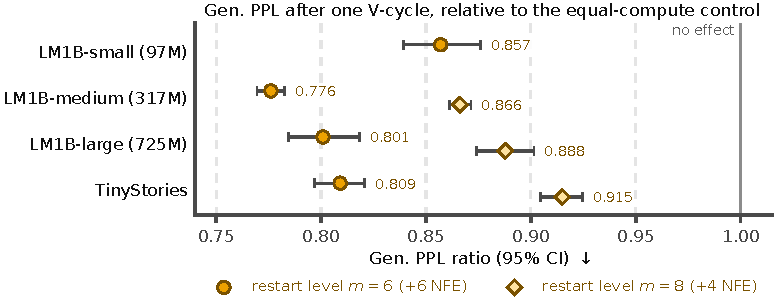
\includegraphics[width=0.8\linewidth]{figures/fig_text.pdf}
\caption{\textbf{One V-cycle against its control.} Generative perplexity after one V-cycle relative to the equal-compute control, for every released LM1B model
and TinyStories, from two restart levels. Bars are paired bootstrap intervals over samples. Restart level 8 was not
run on LM1B-small with three seeds.}
\label{fig:text}
\end{figure}

\paragraph{Restart level and iteration.} On LM1B-small, restarts from levels 4, 6, 8 and 10 all help; a restart from
level 3 does not. Further cycles keep lowering perplexity in smaller steps. On LM1B-medium (seed 42, 256 samples), six
cycles from level 8 reach 65.1 while 95\% of the tokens stay in place from one cycle to the next. Six cycles from
level 6 keep rewriting the draft (70\% of the tokens stay) and end at 51.9, below the perplexity of human text (53.5).
A perplexity below that of human text is not better text, so one cycle is the safe default.

\paragraph{Against temperature.} Lowering the sampling temperature costs nothing and also lowers perplexity, at the
price of diversity, so it is the baseline to beat. In a second run on other hardware (three seeds of 256 samples per
model), we sampled every model at five temperatures from 1 to 0.8 and compared each decoder with the temperature curve
at the decoder's own corpus distinct-2 (Table~\ref{tab:frontier}). The V-cycle repeats its gain over the control there
(ratios of 0.840, 0.784, 0.789 and 0.814 for LM1B-small, medium, large and TinyStories), and its perplexity is 8--13\%
below the temperature curve at equal diversity on all four models. This run was not scored with MAUVE.

\paragraph{Cost.} Evaluations understate what a cycle costs, because the fine levels are the long ones. On LM1B a cycle
from level 6 runs 6 of 11 evaluations but 520 of the 640 code positions of a pass, 81\%. The control pays the same.

\paragraph{Mechanism.} Most of the generator's coarse codes differ from the codes the encoder assigns to the text they
decode to: averaged over the kept levels, 69--97\% of the codes differ (10th--90th percentile of samples, across
models). The control shows that replacing them carries the effect. This is consistent with a training-free correction of exposure bias, but
it does not prove it: the per-sample size of the round trip predicts the gain only weakly (Spearman $\rho\le0.04$ on
LM1B, 0.18 on TinyStories).

\subsection{Prompted tasks}

On translation and summarization the V-cycle is a small polish. On WMT14 the best setting tried, three cycles from
level 3 ($+24$ evaluations), adds $+0.55$ [$+0.25$, $+0.83$] BLEU; a restart from level 7 adds nothing. On XSum three
cycles from level 5 ($+12$ evaluations) add $+0.25$ [$+0.19$, $+0.31$] ROUGE-2 and lower the perplexity of the
summaries by 24\% at unchanged length. These are the best of the restart levels and numbers of cycles tried, on the
test set, and the WMT14 gain is partly selection: a second run repeats it on newstest2014 ($+0.59$ [$+0.29$,
$+0.89$]), but on newstest2013 the same setting gains only $+0.26$ [$-0.05$, $+0.57$]. On WMT14 that is less than half of what guidance adds ($+1.23$ at $+10$ evaluations), on XSum it is more
than guidance adds ($+0.13$ ROUGE-2 at $+8$), and on both it is far below soft decisions, which cost nothing
(Section~\ref{sec:results}). Here the single pass is its own control: regenerating the same levels greedily without
re-encoding reproduces it exactly. One detail matters. The output is re-encoded in canonical form, the text followed
by the end token and padding; re-encoding the raw decoded sequence instead costs $-4.28$ [$-4.77$, $-3.81$] BLEU on
WMT14.

% ------------------------------------------------------------------------------------------------------------------
\section{Results: soft decisions}
\label{sec:results}

\subsection{Translation}

Soft decisions add $+3.48$ BLEU, $+3.4$ chrF and $+3.69$ COMET to the single pass at the same 11 evaluations
(Table~\ref{tab:wmt}). Guidance, at 21 evaluations, adds $+1.23$ BLEU. In lowercased BLEU, soft decisions reach
26.1: above the NCM paper's guidance (23.9 at 22 evaluations) and above its minimum-Bayes-risk decoding (25.2 at
132 evaluations; Figure~\ref{fig:wmt}b). If the paper's scores were cased after all, soft decisions (25.2 cased)
would still match minimum Bayes risk at one twelfth of the evaluations. The paper also lists an autoregressive
baseline at 25.2 with 64 evaluations, taken from earlier work; its scoring protocol may differ, so we show it for
orientation only. The two levers combine, less than additively: soft decisions with a weaker guidance ($s=0.5$) reach 25.52 BLEU and
75.38 COMET.

\begin{table}[t]
\centering
\small
\renewcommand{\arraystretch}{1.12}
\setlength{\tabcolsep}{3.2pt}
\resizebox{\linewidth}{!}{%
\begin{tabular}{lrcccccc}
\toprule
Method & NFE & BLEU & BLEU (lc) & chrF & COMET & $\Delta$ BLEU [95\% CI] & $\Delta$ COMET [95\% CI] \\
\midrule
Single pass (released) & 11 & 21.73 & 22.63 & 49.59 & 70.47 & -- & -- \\
Guidance, $s{=}1$ & 21 & 22.96 & 23.85 & 51.53 & 72.52 & $+1.23$ [$+0.93$, $+1.54$] & $+2.06$ [$+1.74$, $+2.39$] \\
\rowcolor{oursrow} \textbf{Soft decisions}, $T_s{=}1$ & \textbf{11} & \textbf{25.21} & \textbf{26.14} & \textbf{52.99} & \textbf{74.15} & $\mathbf{+3.48}$ [$+3.06$, $+3.84$] & $\mathbf{+3.69}$ [$+3.34$, $+4.02$] \\
Soft + guidance, $s{=}0.5$ & 21 & 25.52 & 26.54 & 53.72 & 75.38 & $+3.79$ [$+3.35$, $+4.17$] & $+4.91$ [$+4.59$, $+5.25$] \\
Min.\ Bayes risk, our run & 132 & 23.44 & 24.28 & 50.49 & -- & $+1.72$ [$+1.35$, $+2.08$] & -- \\
Min.\ Bayes risk over soft candidates & 132 & 24.58 & 25.53 & 51.82 & -- & $+2.86$ [$+2.49$, $+3.23$] & -- \\
\midrule
\emph{NCM paper: guidance} & \emph{22} & & \emph{23.9} & & & & \\
\emph{NCM paper: min.\ Bayes risk} & \emph{132} & & \emph{25.2} & & & & \\
\emph{NCM paper: autoregressive} & \emph{64} & & \emph{25.2} & & & & \\
\bottomrule
\end{tabular}}
\caption{\textbf{Soft decisions on translation.} WMT14 German$\to$English, all 3,003 sentences of newstest2014, greedy decoding. $T_s$ and the guidance scales
were chosen on newstest2013. Differences are against the single pass (paired bootstrap over sentences). The two
minimum-Bayes-risk rows are our own run with 12 sampled candidates, from the second run, whose single pass scores
21.72; COMET was not computed for them. The last three
rows are quoted from the NCM paper and placed under lowercased BLEU (Section~\ref{sec:setup}); its autoregressive
baseline is taken there from earlier work. The proposed setting is highlighted.}
\label{tab:wmt}
\end{table}

On newstest2013 the gain grows with the temperature up to 1 ($+1.4$, $+2.5$, $+3.3$ and
$+3.7$ BLEU at $T_s=0.25$, 0.5, 0.75 and 1) and then turns ($+2.2$ at 1.25, $-6.0$ at 1.5; Figure~\ref{fig:wmt}a). The
best value is the one that needs no tuning: the generator's own distribution.

\begin{figure}[t]
\centering
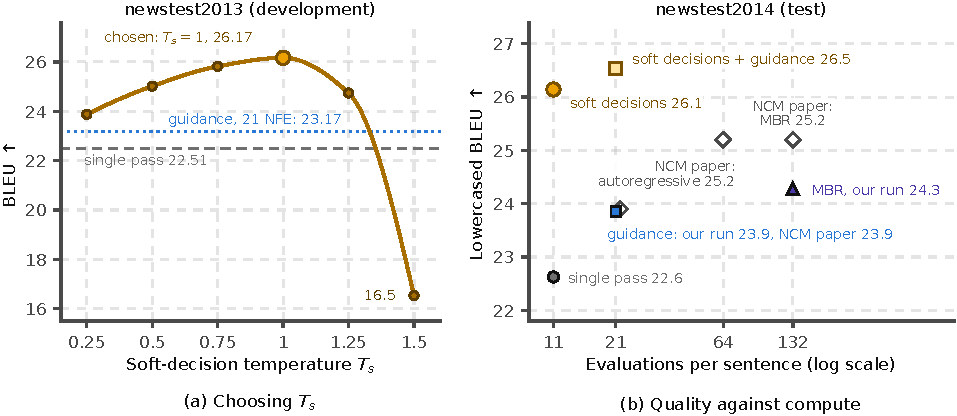
\includegraphics[width=\linewidth]{figures/fig_wmt14.pdf}
\caption{\textbf{Temperature and compute on WMT14.} (a) BLEU on the development set against the soft-decision temperature. The gain
grows up to $T_s=1$, the generator's own distribution, falls off beyond it and collapses at 1.5. (b) Lowercased BLEU
on newstest2014 against generator evaluations per sentence. Filled markers are our runs of the released checkpoint;
open diamonds are quoted from the NCM paper (its autoregressive baseline comes from earlier work).}
\label{fig:wmt}
\end{figure}

\paragraph{Not just length.} The single pass is 6\% too short. Soft decisions raise the length ratio (in words) from 0.938 to
0.989 (brevity penalty 0.928 to 0.978) and the geometric-mean $n$-gram precision from 23.4 to 25.8, so about a third
of the BLEU gain is length and two thirds precision. COMET, which does not count $n$-grams, improves on 65\% of the
sentences. Adjacent repeated words are as rare as before (2.5\% of words before, 2.6\% after).

Averaged over the two orders in which it reads a pair, the LLM judge prefers the
soft-decision translation to the single pass on 66\% of sentences (mean preference 0.633 [0.622, 0.645]) and to the guided translation on 57\% (0.573 [0.562,
0.584]).

For example, the single pass writes ``passengers must off off smart phones, bags and other equipment when
aircraft doors are closed down''; with soft decisions it writes ``passengers have to switch off smart phones, bags and
other equipment when aircraft doors are closed''. ``The Lakes Monkeys must cancel the show at the Hydroiani in
Glasgow'' becomes ``the Arctic Monkeys must also cancel the show at Hydro in Glasgow''.

\paragraph{Our own minimum-Bayes-risk run.} The NCM paper does not state the similarity function or the sampling
temperature of its minimum-Bayes-risk decoding, and the released code has no script for it, so we ran our own: 12
sampled candidates per sentence (132 evaluations), keeping the one with the highest mean similarity to the others,
with the temperature (1 or 0.7) and the similarity (sentence BLEU or chrF) chosen on newstest2013. On newstest2014 it
reaches 23.44 BLEU (24.28 lowercased): $+1.72$ [$+1.35$, $+2.08$] over the single pass, and $-1.77$ [$-2.13$,
$-1.40$] against one soft pass at a twelfth of the cost. That is below the 25.2 of the NCM paper, whose recipe we
could not match; at temperature 1 our run falls below the single pass ($-1.36$ [$-1.78$, $-0.95$]). Selecting among
candidates decoded with soft decisions (coarse levels sampled, the other levels soft) reaches 24.58, still $-0.63$
[$-1.00$, $-0.28$] against the single soft pass. The best of the twelve candidates would score 28.0 and 29.7 in the
two cases: the candidates contain better translations than the selection finds.

\subsection{Summarization}

On XSum the gain is smaller and the temperature matters more (Table~\ref{tab:xsum}). At $T_s=1$ ROUGE rises most, but
the summaries become 17\% shorter and their perplexity rises from 83 to 93: the blend buys ROUGE with terser, less
fluent text. At $T_s=0.5$ the perplexity is unchanged and the summaries lose about one word, so we fixed that value. On
the 5,334 articles that no choice had seen, ROUGE-1/2/L rise by $+0.99$ [$+0.77$, $+1.19$], $+0.84$ [$+0.64$,
$+1.02$] and $+1.16$ [$+0.95$, $+1.34$], and the judge prefers the soft-decision summary (mean preference 0.566
[0.553, 0.578], 2,000 articles). Guidance at twice the cost gains $+0.30$ ROUGE-1 on the same articles and raises the
perplexity to 93. Minimum-Bayes-risk decoding remains stronger here: the NCM paper reports $+2.3$ ROUGE-1 for it at
128 evaluations, and soft decisions recover about two fifths of that at no cost.

\begin{table}[t]
\centering
\small
\renewcommand{\arraystretch}{1.12}
\setlength{\tabcolsep}{6.5pt}
\begin{tabular}{@{}lrccccc@{}}
\toprule
Method & NFE & ROUGE-1 & ROUGE-2 & ROUGE-L & Gen.\ PPL & Words \\
\midrule
Single pass (released) & 9 & 34.92 & 12.71 & 27.93 & 82.6 & 20.7 \\
Guidance, $s{=}0.5$ & 17 & 35.20 & 12.84 & 28.11 & 93.5 & 20.6 \\
\rowcolor{oursrow} \textbf{Soft decisions}, $T_s{=}0.5$ & \textbf{9} & \textbf{35.87} & \textbf{13.52} & \textbf{29.01} & \textbf{81.9} & 19.5 \\
Soft decisions, $T_s{=}1$ & 9 & 36.17 & 13.87 & 29.59 & 93.3 & 17.1 \\
\midrule
\emph{NCM paper: single pass} & & \emph{35.0} & \emph{12.8} & \emph{28.0} & & \\
\emph{NCM paper: guidance} & & \emph{35.3} & \emph{13.0} & \emph{28.2} & & \\
\emph{NCM paper: minimum Bayes risk} & \emph{128} & \emph{37.3} & \emph{14.0} & \emph{29.6} & & \\
\bottomrule
\end{tabular}
\caption{\textbf{Soft decisions on summarization.} XSum, all 11,334 test articles (ROUGE F1), greedy decoding. $T_s$ was fixed on 6,000 of the articles; the
differences in the text are on the other 5,334. Gen.\ PPL is the perplexity of the summaries under GPT-2. The
last three rows are quoted from the NCM paper. The proposed setting is highlighted.}
\label{tab:xsum}
\end{table}

\subsection{Sudoku in one pass}

Sudoku has one right answer per board, so a gain here cannot come from length or style. The released hard-Sudoku model
solves 86.15\% of 2,000 boards in one pass. With soft decisions at $T_s=4$ it solves 89.90\%: 91 boards are repaired
and 16 broken (Table~\ref{tab:sudoku}). On the held-out half the gain is $+3.80$ points [$+2.40$, $+5.00$], from 88.2\%
to 92.0\%. Medium boards gain $+1.50$ [$+0.50$, $+2.60$]; easy boards are solved either way. The best temperature is
higher than on text, and the cliff is as sharp: at $T_s=8$ the hard model solves 22\% of the boards.
Section~\ref{sec:sudoku} adds the V-cycle and spends further evaluations on retries.

\begin{table}[t]
\centering
\small
\renewcommand{\arraystretch}{1.12}
\begin{tabular*}{\linewidth}{@{\extracolsep{\fill}}lcccccl@{}}
\toprule
 & Hard decisions & \multicolumn{4}{c}{Soft decisions, all 2,000 boards (\%)} & Held-out gain of the \\
Difficulty & (\%) & $T_s{=}1$ & $T_s{=}2$ & $T_s{=}4$ & $T_s{=}8$ & chosen $T_s$ [95\% CI] \\
\midrule
Easy & 99.40 & 99.40 & 99.55 & 99.55 & 48.55 & $T_s{=}1$: \phantom{$+$}0.00 [$-0.40$, $+0.40$] \\
Medium & 96.40 & 97.50 & 97.90 & 97.75 & \phantom{0}7.90 & $T_s{=}4$: $+1.50$ [$+0.50$, $+2.60$] \\
Hard & 86.15 & 88.15 & 88.85 & \textbf{89.90} & 22.35 & $T_s{=}4$: $\mathbf{+3.80}$ [$+2.40$, $+5.00$] \\
\bottomrule
\end{tabular*}
\caption{\textbf{Soft decisions on Sudoku, one pass.} Released checkpoints, boards solved exactly in one pass (12 evaluations), 2,000 boards per difficulty.
$T_s$ was chosen on boards 0--999; the last column is the gain of the chosen $T_s$ over hard decisions on boards
1,000--1,999 (paired bootstrap over boards). On easy boards the three lower temperatures tie on boards 0--999 and the
lowest is taken.}
\label{tab:sudoku}
\end{table}

% ------------------------------------------------------------------------------------------------------------------
\section{The full cycle}
\label{sec:full}

The two changes meet in three places: on unconditional text, on the prompted tasks, and on hard Sudoku.

\subsection{Unconditional text}

Under sampling, soft decisions need care. A soft level passes on its mean whatever code was drawn, so with soft
decisions at every level only the draw of level 0 is left: on LM1B, corpus distinct-2 falls from 0.50--0.58 to
0.17--0.19 and perplexity rises by a factor of 2 to 24. Soft decisions at the coarse levels only are worse still, at 5
to 32 times the perplexity of the single pass on the four models: the sampled fine levels cannot follow a blurred
plan. At the fine levels only (level 6 and above, with the coarse levels sampled as released) they act like a lower
temperature, between 6\% below and 9\% above the temperature curve (Table~\ref{tab:frontier}).

The combination is what pays. A V-cycle whose regenerated levels use soft decisions is about a fifth below the
temperature curve at equal diversity on the three LM1B models (ratios of 0.78, 0.81 and 0.81) and a tenth below on
TinyStories (0.91), against 8--13\% for the hard V-cycle.
Against the hard V-cycle itself its perplexity ratio is 0.80, 0.87, 0.88 and 0.98 on the four models. It is the best
decoder we tested on unconditional text.

\begin{table}[t]
\centering
\small
\renewcommand{\arraystretch}{1.12}
\begin{tabular*}{\linewidth}{@{\extracolsep{\fill}}lcccc@{}}
\toprule
 & V-cycle / control & \multicolumn{3}{c}{Perplexity relative to the temperature curve at equal diversity} \\
\cmidrule(l){3-5}
Model & & V-cycle & Soft, fine levels & Soft V-cycle \\
\midrule
LM1B-small & 0.840 [0.820, 0.861] & 0.915 [0.892, 0.932] & 0.940 [0.915, 0.971] & \textbf{0.775} [0.750, 0.794] \\
LM1B-medium & 0.784 [0.766, 0.801] & 0.875 [0.851, 0.888] & 1.085 [1.059, 1.124] & \textbf{0.810} [0.787, 0.821] \\
LM1B-large & 0.789 [0.772, 0.807] & 0.872 [0.847, 0.888] & 1.047 [1.022, 1.084] & \textbf{0.811} [0.786, 0.822] \\
TinyStories & 0.814 [0.803, 0.825] & 0.916 [0.886, 0.931] & 0.943 [0.925, 0.973] & \textbf{0.905} [0.878, 0.920] \\
\bottomrule
\end{tabular*}
\caption{\textbf{Unconditional text against temperature tuning.} Second run, 3 seeds $\times$ 256 samples per model.
\emph{V-cycle / control}: generative perplexity of one cycle from level 6 over that of its equal-compute control. The
other columns divide a decoder's perplexity by that of the temperature curve ($T$ from 1 to 0.8) at the decoder's own
corpus distinct-2; below 1 is better than lowering the temperature. \emph{Soft, fine levels}: soft decisions from
level 6 on, coarse levels sampled. \emph{Soft V-cycle}: a V-cycle from level 6 whose regenerated levels use soft
decisions. Bootstrap over samples within seeds.}
\label{tab:frontier}
\end{table}

\subsection{Translation and summarization}

On translation the two changes do not add up. Starting from the soft pass, a V-cycle with soft regeneration is a tie
on newstest2014 ($+0.17$ [$-0.05$, $+0.42$] BLEU after three cycles from level 3, $-0.04$ [$-0.20$, $+0.11$] after
one cycle from level 5) and slightly negative on newstest2013 ($-0.29$ [$-0.52$, $-0.04$] and $-0.15$ [$-0.29$,
$+0.01$]). The controls say more than the tie. Keeping the soft pass's own chosen codes at the coarse levels, without
re-encoding, loses $-1.08$ [$-1.39$, $-0.75$] below level 3 and $-1.62$ [$-1.92$, $-1.31$] below level 5: once the
plan is hardened to the generator's first choices, part of what the blend gained is gone. Re-encoding the draft also
gives hard coarse codes, and those lose nothing. The encoder's codes for the text are a better discrete plan than
the generator's own first choices.

On summarization the two add a little. On the 5,334 held-out XSum articles, one cycle from level 5 after the soft pass
($+4$ evaluations) adds $+0.21$ [$+0.13$, $+0.30$] ROUGE-2, with $+0.11$ [$+0.02$, $+0.20$] ROUGE-1 and $+0.10$
[$+0.02$, $+0.17$] ROUGE-L, and on the full test set it lowers the perplexity of the summaries from 82 to 61 at
unchanged length. All six settings tried gain between $+0.21$ and $+0.28$ ROUGE-2 on these articles. Soft decisions
and three cycles together are $+1.09$ [$+0.89$, $+1.28$] ROUGE-2 above the single pass.

\subsection{Hard Sudoku with retries}
\label{sec:sudoku}

\begin{table}[t]
\centering
\small
\renewcommand{\arraystretch}{1.12}
\setlength{\tabcolsep}{9pt}
\begin{tabular}{@{}lcc@{}}
\toprule
Method & NCM alone & With singles propagation \\
\midrule
Best-of-$N$ (fresh restarts, $T{=}1$) & 87.9 / 89.5 / 91.4 & 93.6 / 94.5 / 95.7 \\
V-cycle retries, level 5 & 88.6 / 90.2 / 92.0 & 94.1 / 94.8 / 95.6 \\
Fresh greedy restarts in random symmetry frames & 89.7 / 92.8 / 96.1 & 94.9 / 96.4 / 97.8 \\
Symmetry-twisted V-cycle & 91.7 / 94.8 / 97.4 & 95.6 / 97.2 / 98.5 \\
\rowcolor{oursrow} \textbf{Soft decisions + symmetry-twisted V-cycle} & \textbf{94.1 / 96.5 / 98.2} & \textbf{96.8 / 97.9 / 98.8} \\
\bottomrule
\end{tabular}
\caption{\textbf{The full cycle on hard Sudoku.} Released checkpoint: boards solved (\%) at a mean budget of 13 / 14 / 16 generator evaluations
per board (3 seeds $\times$ 2,000 boards). A solution-blind rule checker decides which boards are retried in every
row. \emph{Singles propagation} fills naked and hidden singles from the clues before any retry, at no generator
evaluation, and is accepted only when it completes the grid (85\% of the boards). The soft-decision temperature
($T_s=4$) was chosen on boards 0--999. Budgets count evaluations; at matched FLOPs the first two rows swap order (see
text).}
\label{tab:hard}
\end{table}

\begin{figure}[t]
\centering
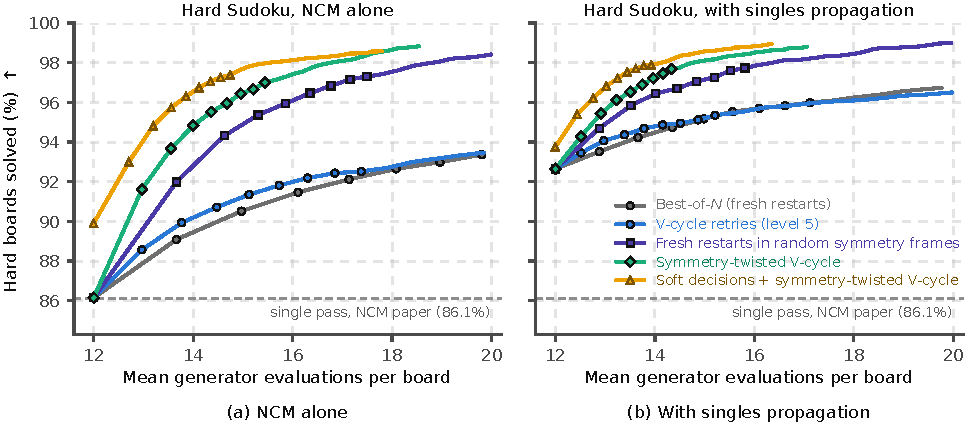
\includegraphics[width=\linewidth]{figures/fig_hard.pdf}
\caption{\textbf{Retries on hard Sudoku.} Released model: boards solved against mean generator evaluations per board, (a) NCM alone with a
rule checker deciding retries, (b) with singles propagation tried before any retry. One point per retry round (markers
on the first eight); 3 seeds $\times$ 2,000 boards.}
\label{fig:hard}
\end{figure}

A rule checker can tell a wrong board from a right one without the solution, so on Sudoku a decoder can retry. We compare five ways to spend the retries at the same mean number of evaluations per board (Table~\ref{tab:hard},
Figure~\ref{fig:hard}). The restart level and the other retry settings were fixed without separate data. Two things
carry most of the gain: a new symmetry frame for every retry, and soft decisions. The differences that follow are for
NCM alone, on the held-out boards at 14 evaluations. Fresh greedy restarts in random frames beat
best-of-$N$ by $+2.73$ [$+1.86$, $+3.50$], because retries stop repeating rejected boards (duplicates 11\% against
35\%); the two arms differ in the frame and in greedy against sampled decoding. Soft decisions add $+1.65$ [$+0.69$,
$+2.58$] to the twisted V-cycle, and the full stack gains $+5.16$ [$+3.80$, $+6.38$] over fixed-frame V-cycle retries.

\paragraph{The share of re-encoding.} Re-encoding adds little here. In a separate run with sampled retries in a fixed frame, a V-cycle from
level 5 is within noise of its no-restriction control ($+0.27$ [$-0.20$, $+0.71$] at 14 evaluations, all boards); from
level 7 it is ahead ($+0.67$ [$+0.20$, $+1.21$]). Keeping the re-encoded coarse levels in a new frame adds $+1.25$
[$+0.34$, $+2.09$] over a fresh restart in a new frame at equal evaluations, but a level-5 retry processes most of the
code positions while counting as 7 of 12 evaluations. At matched FLOPs (1.2 full passes, all boards), V-cycle retries
are slightly below best-of-$N$ ($-0.50$ [$-1.04$, $-0.02$]) and the twisted V-cycle ties random-frame restarts
($-0.38$ [$-0.91$, $+0.07$]). We did not run soft decisions with random frames and no re-encoding, so the share of
re-encoding in the best row is not isolated. On these unique-solution puzzles the rule checker is an exact verifier,
so the numbers measure how often a correct board is produced within the budget.

\paragraph{Error detection.} Without the solution, the level-local residual detects wrong boards with
an AUROC of 0.92 (plain round-trip residual 0.86, decoder confidence 0.87).

% ------------------------------------------------------------------------------------------------------------------
\section{Analysis of soft decisions}
\label{sec:analysis}

\subsection{Where soft decisions act}

Figure~\ref{fig:levels} applies soft decisions to subsets of the levels. On WMT14 at $T_s=1$, the five coarsest levels
alone (47 of 313 code positions) give $+2.2$ of the $+3.5$ BLEU, and every level but the last gives $+3.3$. Most of the
effect is in the plan; the fine levels add the rest. On XSum the coarse levels alone (levels 0--3 of 9) help at $T_s=0.5$ but not at
$T_s=1$, where the gain needs the fine levels as well.

\begin{figure}[t]
\centering
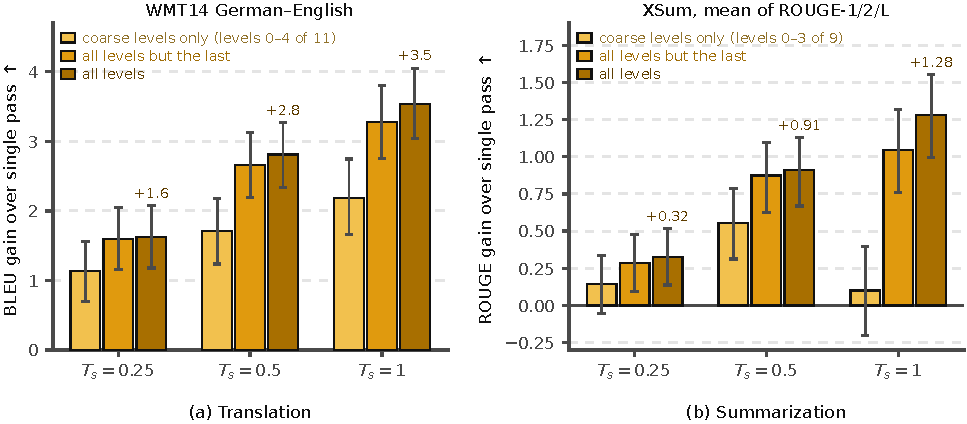
\includegraphics[width=\linewidth]{figures/fig_levels.pdf}
\caption{\textbf{Where soft decisions act.} Gain over the single pass when soft decisions are applied to the coarse levels only, to all levels but the
last, or to all levels (first run, report half: 1,502 WMT14 sentences and 3,000 XSum articles; bars are paired
bootstrap intervals). $T_s=2$ collapses in every variant (Appendix~\ref{app:grid}).}
\label{fig:levels}
\end{figure}

\subsection{The blend, not a code}

If the posterior mean merely pointed at a better code, we could pick that code and keep hard decisions.
Table~\ref{tab:variants} says otherwise.

\begin{table}[t]
\centering
\small
\renewcommand{\arraystretch}{1.12}
\begin{tabular*}{\linewidth}{@{\extracolsep{\fill}}P{6.2cm}cc@{}}
\toprule
Variant & $\Delta$ BLEU vs.\ single pass & $\Delta$ BLEU vs.\ soft decisions \\
\midrule
Soft decisions, all levels, $T_s{=}1$ & $+3.54$ [$+3.01$, $+4.08$] & -- \\
Soft decisions, levels 0--4 only & $+2.19$ [$+1.66$, $+2.70$] & $-1.35$ [$-1.67$, $-1.01$] \\
\midrule
Nearest code, levels 0--4, $T_s{=}0.5$ & $-1.22$ [$-1.72$, $-0.70$] & $-4.75$ [$-5.30$, $-4.24$] \\
Nearest code, levels 0--4, $T_s{=}1$ & $-10.37$ [$-11.21$, $-9.55$] & \\
Nearest code, all levels, $T_s{=}1$ & $-15.08$ [$-15.84$, $-14.33$] & \\
\midrule
Confidence gate, $\tau{=}0.3$ & $+2.24$ [$+1.74$, $+2.78$] & $-1.29$ [$-1.71$, $-0.88$] \\
Confidence gate, $\tau{=}0.5$ & $+3.01$ [$+2.48$, $+3.58$] & $-0.53$ [$-0.82$, $-0.24$] \\
Confidence gate, $\tau{=}0.9$ & $+3.51$ [$+3.00$, $+4.06$] & $-0.03$ [$-0.08$, $+0.03$] \\
\midrule
Top-2 blend, $T_s{=}1$ & $+1.90$ [$+1.41$, $+2.39$] & $-1.64$ [$-2.12$, $-1.17$] \\
Top-8 blend, $T_s{=}1$ & $+3.42$ [$+2.92$, $+3.95$] & $-0.12$ [$-0.51$, $+0.21$] \\
Top-16 blend, $T_s{=}1$ & $+3.74$ [$+3.23$, $+4.29$] & $+0.20$ [$-0.14$, $+0.52$] \\
Top-8 blend, $T_s{=}2$ & $+3.75$ [$+3.19$, $+4.34$] & $+0.21$ [$-0.18$, $+0.58$] \\
\bottomrule
\end{tabular*}
\caption{\textbf{Variants of soft decisions.} WMT14, report half of newstest2014 (1,502 sentences; paired bootstrap).
\emph{Nearest code} re-quantizes the posterior mean to the closest codebook vector. \emph{Confidence gate} takes the
argmax wherever the top probability is at least $\tau$ and stays soft elsewhere. \emph{Top-$k$} blends only the $k$
most probable codes. The first two rows repeat arms of Appendix~\ref{app:grid} in a second run with its own bootstrap, so
their intervals differ from the appendix in the second decimal.}
\label{tab:variants}
\end{table}

\paragraph{Nearest code.} Re-quantizing the posterior mean to its nearest code is worse than the
single pass at every temperature, and collapses at $T_s=1$ ($-10.4$ BLEU on the coarse levels alone, $-15.1$ on all
levels). The nearest code is often not the argmax (at $T_s=1$ it changes 24--98\% of the codes of the five coarse levels), and
it decodes to much shorter text (brevity penalty 0.52). The information is in the mixture.

\Needspace{6\baselineskip}% as for "Plan swaps" below: do not resume under the table of the next page
\paragraph{Confidence gate.} Taking the argmax wherever the generator is confident loses $1.3$ BLEU at
a threshold of 0.3 and only ties with plain soft decisions at 0.9, where a quarter of the positions are still committed, most of them
at the fine levels. SeLaR \citep{selar2026} reports gains for autoregressive reasoning models from soft inputs at uncertain steps only;
on NCM the same kind of gate never beats staying soft.

\paragraph{Top-$k$ blends.} Blending only the two most probable codes keeps half of the gain; eight codes
keep nearly all of it. Truncating the blend also removes the collapse at high temperature: a top-8 blend at $T_s=2$
was the best variant on the tuning half, but against plain soft decisions it is a tie in BLEU on the report half
($+0.21$ [$-0.18$, $+0.58$]) and on newstest2013 ($-0.05$ [$-0.35$, $+0.24$]), with a small gain
in COMET on all sentences of newstest2014, tuning half included, and of newstest2013 ($+0.90$ [$+0.63$, $+1.18$] and
$+0.41$ [$+0.16$, $+0.67$]). We keep the plain blend.

\paragraph{High temperature.} At $T_s=2$ the plain blend fails on every subset of levels:
WMT14 output becomes twice too long and BLEU falls to 0.6; XSum summaries shrink to 8 words
(Appendix~\ref{app:grid}).

% ------------------------------------------------------------------------------------------------------------------
\section{Why a blend helps: the plan is a model error}
\label{sec:why}

Which part of NCM costs the points on translation? The measurements in this section train nothing and decode greedily.

\paragraph{Tokenizer ceiling.} The tokenizer is not the bottleneck. References cut to the model's output length and passed through the
frozen tokenizer come back at 95.5 BLEU (99.4\% of tokens), and at 99.5 ROUGE-1 on the first 3,000 XSum test articles.

% keep this paragraph whole: when it started in the last lines of a page, it resumed under the table of the next one
\Needspace{6\baselineskip}
\paragraph{Plan swaps.} The coarse plan is. We take the output of a stronger German$\to$English system, encode it with the frozen
tokenizer, give NCM its levels 0--4 in place of NCM's own (47 of 313 code positions), and let NCM generate the other
levels with the same prompt. With the plan of OPUS-MT \citep{tiedemann2020opusmt} NCM reaches 28.08 BLEU, and with the
plan of the WMT19 system of \citet{ng2019fair} 30.47 (Table~\ref{tab:plans}). Five coarse levels close half of the
BLEU gap to the system they come from, for both systems on both test sets, and a third or more of the COMET gap (33--39\%). NCM's fine
levels are able to write a much better translation than its own coarse levels ask for.
Appendix~\ref{app:plans} varies the number of levels taken from the plan.

\begin{table}[t]
\centering
\small
\renewcommand{\arraystretch}{1.12}
\setlength{\tabcolsep}{3.5pt}
\begin{tabular*}{\linewidth}{@{\extracolsep{\fill}}llC{1.15cm}C{1.45cm}C{0.95cm}C{1.75cm}C{1.2cm}C{1.35cm}C{1.5cm}@{}}
\toprule
 & & \multicolumn{3}{c}{BLEU} & \multicolumn{4}{c}{The plan's levels 0--4 under NCM's generator} \\
\cmidrule(lr){3-5}\cmidrule(lr){6-9}
Plan from & Test set & System alone & NCM with the plan & Share of gap & Sentences where NCM scores it higher & Median rank, level 0 & Median rank, levels 1--4 & In NCM's top 5, levels 1--4 \\
\midrule
OPUS-MT & newstest2014 & 33.93 & 28.08 & 52\% & 0.4\% & 8 & 0--1 & 85--94\% \\
 & newstest2013 & 31.95 & 27.58 & 54\% & 0.6\% & 6 & 0 & 87--95\% \\
WMT19 system & newstest2014 & 39.32 & 30.47 & 50\% & 0.2\% & 10 & 0--1 & 83--93\% \\
 & newstest2013 & 36.49 & 29.82 & 52\% & 0.5\% & 7 & 0--1 & 86--94\% \\
\bottomrule
\end{tabular*}
\caption{\textbf{A better plan under NCM's own generator.} WMT14. \emph{NCM with the plan}: BLEU when levels 0--4 come from the
system's output and NCM generates the rest. \emph{Share}: that gain as a fraction of the gap between NCM's single pass
(21.73 on newstest2014, 22.5 on newstest2013) and the system alone. The last four columns score the plan's levels
0--4 with NCM's generator (teacher-forced) against NCM's own greedy plan.}
\label{tab:plans}
\end{table}

\paragraph{Search or model error.} If NCM ranked the better plan above its own and merely failed to reach it, a better
search would help. It does not. Scored level by level with NCM's own generator, the other system's levels 0--4 rank
below NCM's greedy levels in 99.4--99.8\% of sentences: a model error, not a search error, in the sense of
\citet{stahlberg2019nmt}. NCM's score also cannot tell when the other plan would help. The plan improves chrF for
66--74\% of sentences, but the score gap predicts which ones with an AUROC of 0.48--0.50, and keeping the other plan
only where NCM prefers it changes chrF by at most $+0.11$. Reranking candidates by NCM's likelihood has nothing to
find.

\paragraph{Where the better codes rank.} Yet the better codes are close. Position by position, the better plan sits near the top of NCM's
distributions. At levels 1--4 its codes are NCM's argmax in 46--65\% of the positions and within NCM's five most
probable codes in 83--95\% of them; the median rank is 0 or 1. Only at level 0, a single code for the whole sentence,
do they rank lower (median 6--10). A hard decision keeps only the top code; wherever the better plan's code is the runner-up, it is
discarded. A posterior mean keeps both, in proportion. This is consistent with soft decisions working where
reranking cannot, and with most of their effect sitting in the coarse levels (Figure~\ref{fig:levels}); it does not
prove that this is the mechanism.

\paragraph{Summarization.} On XSum the first level of a better plan, which settles what the summary is about, lies
far down NCM's list (median rank 122 for the plans of a fine-tuned BART \citep{lewis2020bart}, on the first 3,000 test articles), and soft decisions
help less there. This comparison is confounded, because BART has seen the test summaries (Section~\ref{sec:limits}).

% ------------------------------------------------------------------------------------------------------------------
\section{Related work}
\label{sec:related}

\paragraph{Multigrid and re-encoding.} A coarse-to-fine pass is the prolongation half of a multigrid V-cycle
\citep{brandt1977multigrid,briggs2000multigrid}; restriction is the other half. The closest precedent for
restrict-then-regenerate is the scale-travel step of DiverseVAR \citep{park2025diversevar}, which re-quantizes an
accumulated image latent once at a fixed scale; we restrict through the discrete output and the full encoder, on
text, against an equal-compute control. Random symmetry frames as instance augmentation appear in POMO
\citep{kwon2020pomo}.

\paragraph{Soft decisions in decoding.} In iterative (turbo) decoding, later stages receive the expected symbol
instead of a hard decision \citep{wang1999iterative}, and soft vector-quantizer decoding reconstructs the
posterior-weighted mean of the code vectors \citep{skoglund1999soft}. Equation~\ref{eq:soft} is that principle,
applied between the levels of a multiscale generator.

\paragraph{Soft inputs in sequence models.} Probability-weighted embeddings have been fed back at inference in flat
token sequences. AiT \citep{ning2023ait} feeds the probability-weighted average of codebook embeddings to the next
autoregressive step and to the VQ decoder of a vision model. Soft Thinking \citep{zhang2025softthinking} feeds the
probability-weighted mixture of token embeddings to a language model while it reasons, without training. Mixture of
Inputs \citep{zhuang2025moi} reports that this pure posterior mean degrades language models in most cases and blends
it with the sampled token instead, and SeLaR \citep{selar2026} uses the mixture only at steps where the model is
uncertain. Continuous-thought models train the network to read its own hidden state \citep{hao2024coconut}. We are not aware of an earlier use of the posterior mean between the levels of a multiscale
(next-scale or residual-VQ) generator \citep{tian2024var,lee2022rqvae}, where the levels are summed into one latent,
and the NCM paper uses hard codes throughout. What we report is the measured effect on NCM, not the principle.

\paragraph{Guidance and risk minimisation.} Classifier-free guidance \citep{ho2022cfg} and minimum-Bayes-risk decoding
\citep{kumar2004mbr,eikema2020map} improve NCM at 2\x\ and 12\x\ the cost in the NCM paper. Soft decisions are
orthogonal to both; we combined them with guidance and did not combine them with minimum Bayes risk.

\paragraph{Plans and model errors.} Oracles built from the reference's own latent codes or plans are common in
non-autoregressive translation and planned summarization \citep{bao2021cnat,narayan2021frost}, and
\citet{dou2021gsum} compare such oracle guidance with guidance predicted by another system. Our plan swaps pass another
system's output through a frozen tokenizer into a frozen generator. The split into search and model errors follows
\citet{stahlberg2019nmt} and the inadequacy of the mode \citep{eikema2020map}; for a non-autoregressive model,
\citet{ma2019flowseq} found its own likelihood a weaker reranker than an external teacher.

% ------------------------------------------------------------------------------------------------------------------
\section{Limitations}
\label{sec:limits}

\begin{itemize}[leftmargin=*, topsep=4pt, itemsep=3pt, parsep=0pt]
\item \emph{Scale and coverage.} Each prompted task has one released checkpoint, of 120M parameters or fewer.
  Whether soft decisions help larger NCM models on prompted tasks is untested. The V-cycle was measured on four
  unconditional models, of 97M to 725M parameters for LM1B.
\item \emph{V-cycles.} A cycle runs the frozen encoder once, which we do not count as a generator evaluation, and a
  cycle from level 6 processes 81\% of the code positions of a pass. One cycle lowers corpus distinct-2 by 3--6\%. The
  comparison with temperature tuning uses three seeds per model and no MAUVE, and the iteration results come from one
  seed. On the prompted tasks the reported V-cycle settings are the best of those tried on the test set, and the
  WMT14 gain is not significant on newstest2013.
\item \emph{Sudoku retries are a hybrid.} They need a rule checker and Sudoku's symmetry group, which free text
  does not have, and their settings were not chosen on separate data. At matched FLOPs, re-encoding adds nothing
  there.
\item \emph{Sampling and minimum Bayes risk.} On the prompted tasks soft decisions were tuned for greedy decoding.
  Under sampling they help only at the fine levels or inside a V-cycle. Our minimum-Bayes-risk run does not reach the
  25.2 BLEU printed in the NCM paper, whose recipe and BLEU casing are not stated (Section~\ref{sec:setup}), so that
  comparison rests on our recipe on one side and on the printed score on the other.
\item \emph{The temperature must be set.} The best $T_s$ was 1 on translation, 0.5 on summarization and 4 on hard
  Sudoku, and too high a value collapses the output. On XSum the choice trades ROUGE against fluency and length.
\item \emph{Selection data.} The NCM release has no XSum development split, so $T_s$ was fixed on 6,000 test
  articles and the differences are reported on the remaining 5,334; the full-test scores of Table~\ref{tab:xsum}
  include the selection articles. On WMT14, newstest2014 was not untouched when $T_s$ was chosen on newstest2013: the
  first run had tried four temperatures on it. On Sudoku, the selection and held-out boards are halves of the same
  2,000.
\item \emph{Hardware.} Decoding is greedy and deterministic on one machine, but many decisions are near-ties. In a
  CPU rerun of the first 32 newstest2014 sentences, five single-pass translations differ from the GPU run, each
  from one code with a logit gap below 0.003.
\item \emph{Evaluation.} There is no human evaluation. The evidence is BLEU, chrF, COMET, ROUGE, perplexity
  scorers, MAUVE and one 7B LLM judge with a strong position bias (it picks the same text in both orders for only about half
  of the pairs).
\item \emph{The diagnosis is not a proof.} The plan swaps measure headroom with another system's output; they are
  not a decoding method. The XSum swap is confounded: BART reaches 67.7 ROUGE-1 on these articles against 45.1 in
  its paper and reproduces 7\% of the references exactly, so it has seen them.
\item \emph{The model was not trained for soft inputs.} All gains are obtained with a generator that only ever saw
  hard codes. Training with soft inputs may help further; we did not test it here.
\end{itemize}

% ------------------------------------------------------------------------------------------------------------------
\section{Conclusion}

An NCM pass is the downward half of a V-cycle, taken once and with hard decisions. Both halves can be had without
training. Going back up, sending a draft through the frozen tokenizer and regenerating its fine levels lowers the
perplexity of unconditional text by 14--22\% against a control of equal compute, and by 8--13\% against temperature
tuning at equal diversity. On the prompted tasks it is a small polish, and on hard Sudoku it adds little, and nothing
at matched FLOPs. Going down, passing on the posterior-mean code vector instead of a committed code costs nothing and
is worth $+3.5$ BLEU on WMT14, more than guidance at 2\x\ the compute and more than our own minimum-Bayes-risk run at
12\x, with smaller gains on summarization and on Sudoku. The diagnosis says why: the better plan is mostly made of the
generator's first and second choices, yet the generator's own likelihood ranks it below its greedy plan, so a hard
decision discards what no reranking can recover. Together, the two give the best unconditional text we measured, a
V-cycle with soft regeneration about a fifth below temperature tuning on LM1B, and with a rule checker and a new
symmetry frame for every retry they take the released hard-Sudoku model from 86.2\% to 96.5\% at 14 evaluations per
board. On translation they do not add up. For a model whose levels add up to one latent, a cycle with soft messages
between its levels is a natural way to decode.

\paragraph{Code and data.} The decoder, the experiment scripts, every result file behind the tables and figures, and
the pinned revisions of the NCM code, checkpoints and datasets are at
\url{https://github.com/maqiaai-lab/ncm-vcycles}. Every experiment runs the released checkpoints; nothing is
trained.

\section*{Acknowledgments}
We thank the authors of Next-Concept Modeling for releasing their code, checkpoints and
data, and Hermann Kumbong, Ishan Khare and Junmiao Hu for discussions.

\clearpage
\bibliographystyle{unsrtnat}
\bibliography{refs}

\clearpage
\appendix

% ------------------------------------------------------------------------------------------------------------------
\section{First run: temperatures and level subsets}
\label{app:grid}

Table~\ref{tab:grid} gives every soft-decision arm of the first run. Documents were split at random into a tuning
half and a report half; the table shows the report half. The first run fixed the design of the confirmation runs of
Section~\ref{sec:results}, where $T_s$ was chosen again on newstest2013.

\begin{table}[H]
\centering
\small
\renewcommand{\arraystretch}{1.12}
\setlength{\tabcolsep}{5pt}
\begin{tabular*}{\linewidth}{@{\extracolsep{\fill}}llcccc@{}}
\toprule
 & & \multicolumn{2}{c}{WMT14} & \multicolumn{2}{c}{XSum} \\
Levels & $T_s$ & $\Delta$ BLEU [95\% CI] & Length & $\Delta$ mean ROUGE [95\% CI] & Words \\
\midrule
All & 0.25 & $+1.62$ [$+1.18$, $+2.07$] & 0.939 & $+0.32$ [$+0.14$, $+0.51$] & 20.3 \\
All but the last & 0.25 & $+1.59$ [$+1.16$, $+2.05$] & 0.938 & $+0.28$ [$+0.10$, $+0.48$] & 20.3 \\
Coarse only & 0.25 & $+1.13$ [$+0.70$, $+1.55$] & 0.938 & $+0.14$ [$-0.06$, $+0.33$] & 20.3 \\
\midrule
All & 0.5 & $+2.81$ [$+2.33$, $+3.27$] & 0.947 & $+0.91$ [$+0.67$, $+1.13$] & 19.5 \\
All but the last & 0.5 & $+2.66$ [$+2.19$, $+3.13$] & 0.948 & $+0.87$ [$+0.62$, $+1.10$] & 19.4 \\
Coarse only & 0.5 & $+1.71$ [$+1.24$, $+2.18$] & 0.946 & $+0.55$ [$+0.31$, $+0.79$] & 19.3 \\
\midrule
All & 1 & $+3.53$ [$+3.04$, $+4.05$] & 0.976 & $+1.28$ [$+1.00$, $+1.56$] & 17.1 \\
All but the last & 1 & $+3.27$ [$+2.76$, $+3.81$] & 0.976 & $+1.05$ [$+0.76$, $+1.32$] & 17.1 \\
Coarse only & 1 & $+2.19$ [$+1.67$, $+2.75$] & 0.976 & $+0.10$ [$-0.20$, $+0.40$] & 16.8 \\
\midrule
All & 2 & $-20.77$ [$-21.54$, $-19.97$] & 2.08 & $-5.46$ [$-5.83$, $-5.10$] & 8.5 \\
All but the last & 2 & $-20.74$ [$-21.49$, $-19.95$] & 2.05 & $-8.03$ [$-8.39$, $-7.63$] & 7.2 \\
Coarse only & 2 & $-19.60$ [$-20.34$, $-18.81$] & 1.69 & $-3.82$ [$-4.20$, $-3.44$] & 11.6 \\
\bottomrule
\end{tabular*}
\caption{\textbf{First run, report half.} WMT14: 1,502 sentences of newstest2014; XSum: 3,000 of 6,000 articles. Differences
against the single pass (21.36 BLEU; 25.02 mean ROUGE-1/2/L), paired bootstrap. \emph{Length}: output length relative
to the reference (WMT14) and words per summary (XSum; single pass 20.6).}
\label{tab:grid}
\end{table}

\section{Plan swaps at other depths}
\label{app:plans}

Table~\ref{tab:depth} varies how many levels come from the plan. The
reference's own codes are not a fair plan: the coarse codes of a reference spell out that very reference, so the
teacher-forced oracle (51.8 BLEU with five levels) overstates the planning gap by a factor of 3.4 to 4.7 against a
plan from another system (30.5 with the WMT19 system's, 28.1 with OPUS-MT's).

\begin{table}[H]
\centering
\small
\renewcommand{\arraystretch}{1.12}
\begin{tabular*}{\linewidth}{@{\extracolsep{\fill}}lcccc@{}}
\toprule
Source of the first $k$ levels & $k=1$ & $k=3$ & $k=5$ & $k=9$ \\
\midrule
OPUS-MT (alone: 33.93) & 22.81 & 24.80 & 28.08 & 31.54 \\
WMT19 system (alone: 39.32) & 22.38 & 25.45 & 30.47 & 36.09 \\
The reference (teacher-forced oracle) & 23.73 & 31.20 & 51.83 & 86.95 \\
\bottomrule
\end{tabular*}
\caption{\textbf{Plan swaps at other depths.} WMT14 newstest2014: BLEU when the first $k$ levels come from a plan and NCM generates the rest (single pass
21.73). In COMET, five levels close 35\% (OPUS-MT) and 33\% (WMT19 system) of the gap to the plan's system, and nine
levels 69\% and 67\%.}
\label{tab:depth}
\end{table}

\end{document}
